% ============================================================
%  Chapter 6 ---'' Type Inference: How the Compiler Reads Your Mind
%  Type Theory from the Ground Up
% ============================================================
\chapter{Type Inference: How the Compiler Reads Your Mind}
\label{ch:type-inference}

\begin{keyinsight}[What This Chapter Is About]
In the previous two chapters we studied polymorphism and System~F.
We wrote types like $\forall \alpha.\, \alpha \to \alpha$ and felt rather pleased
with ourselves.
But we also wrote them \emph{by hand}.
Every binding needed an annotation, every type abstraction needed an
explicit type variable.
That gets old fast.

This chapter is about the question: \emph{can the compiler figure the types out
for us?}
The answer is a qualified, fascinating ``yes''---with some important
caveats.
We will learn how compilers generate \emph{type constraints}, how they
\emph{solve} those constraints with unification, and how the beautiful
Algorithm~W packages this all up into a system that infers the most general
possible type for any expression in a large, useful fragment of typed
lambda calculus.
We will also see where the magic breaks down---and why that breakdown is,
provably, unavoidable.
\end{keyinsight}

% ------------------------------------------------------------
\section{The Annotation Burden}
\label{sec:annotation-burden}
% ------------------------------------------------------------

Let us start by appreciating the problem.

In the Simply Typed Lambda Calculus (STLC) from Chapter~3, every function
argument carries a mandatory type annotation.
You write:
\[
  \lambda x : \mathsf{int}.\; x + 1
\]
That is fine for a single function.
But the moment you start composing functions, the noise accumulates:
\[
  \lambda f : (\mathsf{int} \to \mathsf{int}).\; \lambda x : \mathsf{int}.\; f\,(f\,x)
\]
In System~F (Chapter~5), things get worse.
The identity function looks like this:
\[
  \Lambda \alpha.\; \lambda x : \alpha.\; x
\]
To actually \emph{use} it at type \code{int} you must write:
\[
  (\Lambda \alpha.\; \lambda x : \alpha.\; x)\;[\mathsf{int}]\; 42
\]
Every type instantiation is spelled out explicitly.
System~F is powerful, but writing programs in it by hand is roughly as
pleasant as filling out tax forms.

\begin{intuition}
Think of it this way.
When a friend hands you a thermos and says ``have some,'' you do not stop and
demand to know the precise chemical composition of the liquid.
You look at the context---it is lunchtime, it smells like coffee, they are
carrying a coffee cup---and you \emph{infer} it is coffee.
A type inferencer does the same thing: it looks at the \emph{context in which
a variable is used} and figures out what type it must have.
\end{intuition}

The goal of type inference is to let you write:
\begin{lstlisting}[style=haskell]
-- Haskell: no type annotation needed
double f x = f (f x)
\end{lstlisting}
and have the compiler work out that \code{double} has type
$(\alpha \to \alpha) \to \alpha \to \alpha$ for some type variable $\alpha$,
or more precisely $\forall \alpha.\, (\alpha \to \alpha) \to \alpha \to \alpha$.

That is the promise.
Now let us see how it is kept.

% ------------------------------------------------------------
\section{Type Inference: The Big Idea}
\label{sec:big-idea}
% ------------------------------------------------------------

\begin{definition}[Type Inference Problem]
Given an expression $e$ with no (or partial) type annotations, find a typing
context $\Gamma$ and a type $\tau$ such that $\Gamma \vdash e : \tau$, or
report that no such typing exists.
\end{definition}

The key insight is that type information is not arbitrary---it is
\emph{constrained} by the operations you perform.

Consider the tiny expression $x + 1$.
You do not know the type of $x$ yet.
But you know that $+$ requires both operands to be numbers (let us say
\code{int} for concreteness).
So whatever $x$ is, it had better be \code{int}.

This is the heart of type inference: use the \emph{shape of an expression} to
deduce what types must be.

The process has two phases:
\begin{enumerate}[label=\textbf{Phase \arabic*.}]
  \item \textbf{Constraint Generation.}
        Walk the expression tree.
        Assign fresh type variables to any sub-expression whose type is
        unknown.
        Every language construct generates \emph{equations} between types.
        Collect all those equations.
  \item \textbf{Constraint Solving (Unification).}
        Solve the system of type equations.
        If a solution exists, substitute it back.
        The result is the inferred type.
        If no solution exists, the program has a type error.
\end{enumerate}

\begin{keyinsight}[Inference Is Equation Solving]
Type inference turns a typing problem into algebra.
You have unknowns (fresh type variables) and equations (constraints from
language constructs).
Solving the system is just solving the algebra.
The only trick is that the algebra happens over \emph{types}, not numbers,
so ordinary linear algebra does not apply---we need a specialised algorithm
called \emph{unification}.
\end{keyinsight}

% ------------------------------------------------------------
\section{Constraint Generation: A Step-by-Step Example}
\label{sec:constraint-generation}
% ------------------------------------------------------------

Let us work through the simplest non-trivial example: inferring the type of
\[
  e \;=\; \lambda x.\; x + 1
\]
where $x$ has no annotation.

\subsection{Step 1: Assign Type Variables}

We do not know the type of $x$, so we give it a fresh type variable.
Call it $\alpha$.
Our working assumption:
\[
  x : \alpha
\]
We also do not know what type the whole lambda will have yet.
Call it $\tau$.

\subsection{Step 2: Walk the Body}

The body is $x + 1$.
We need to type-check the application of $+$.

In our language, $+$ has type $\mathsf{int} \to \mathsf{int} \to \mathsf{int}$.
(It takes two ints and returns an int.)

\begin{itemize}
  \item The left operand is $x$, which we said has type $\alpha$.
        For the addition to be well-typed, we need $\alpha = \mathsf{int}$.
        \textbf{Constraint generated:} $\alpha = \mathsf{int}$.
  \item The right operand is $1$, which has type $\mathsf{int}$.
        This is already consistent; no new constraint beyond what we have.
  \item The result of $x + 1$ has type $\mathsf{int}$.
\end{itemize}

\subsection{Step 3: Assemble the Type}

The lambda $\lambda x.\, x + 1$ takes something of type $\alpha$ and returns
something of type $\mathsf{int}$.
So its type is $\alpha \to \mathsf{int}$.

\subsection{Step 4: Solve the Constraints}

We have exactly one constraint: $\alpha = \mathsf{int}$.
Substituting:
\[
  \text{type of } (\lambda x.\, x + 1) \;=\; \alpha \to \mathsf{int}
  \;\xrightarrow{\alpha := \mathsf{int}}\; \mathsf{int} \to \mathsf{int}
\]

The inferred type is $\mathsf{int} \to \mathsf{int}$.
This matches what you would write by hand.

\begin{example}[A Two-Variable Example]
Consider $\lambda x.\, \lambda y.\, x + y$.
\begin{enumerate}
  \item Assign $x : \alpha$, $y : \beta$.
  \item Body $x + y$: both operands of $+$ must be \code{int}.
        Constraints: $\alpha = \mathsf{int}$, $\beta = \mathsf{int}$.
  \item Result of $x + y$ is $\mathsf{int}$.
  \item Type of the whole thing: $\alpha \to \beta \to \mathsf{int}$.
  \item After substitution: $\mathsf{int} \to \mathsf{int} \to \mathsf{int}$.
\end{enumerate}
\end{example}

\begin{example}[The Identity Function]
Now something more interesting: $\lambda x.\, x$.
\begin{enumerate}
  \item Assign $x : \alpha$.
  \item Body is just $x$, so the result type is also $\alpha$.
  \item No operation constrains $\alpha$. The constraint set is \emph{empty}.
  \item Type: $\alpha \to \alpha$.
\end{enumerate}
Since $\alpha$ is unconstrained, it can be \emph{anything}.
The type $\alpha \to \alpha$ is already a polymorphic type: we can
universally quantify it to get $\forall \alpha.\, \alpha \to \alpha$.
\end{example}

\begin{example}[Function Application]
Consider $f\, 42$ where $f$ is some unknown function.
\begin{enumerate}
  \item Assign $f : \phi$ (fresh type variable).
  \item $42$ has type $\mathsf{int}$.
  \item Applying $f$ to $42$ means $\phi$ must be a function type
        $\mathsf{int} \to \rho$ for some fresh $\rho$.
        Constraint: $\phi = \mathsf{int} \to \rho$.
  \item The result type of the application is $\rho$.
\end{enumerate}
\end{example}

These examples hint at a pattern.
Each language construct---lambda, application, let-binding, conditionals,
operators---generates a specific kind of constraint.
Let us collect the constraint generation rules for a simple lambda calculus.

\subsection{The Constraint Generation Rules}

Let $\mathcal{C}(e, \tau)$ mean ``generate constraints that make $e$ have type
$\tau$, given current environment''.
We write $\text{fresh}()$ to mean ``allocate a new type variable never used
before''.

\begin{center}
\renewcommand{\arraystretch}{1.8}
\begin{tabular}{lp{8cm}}
\toprule
\textbf{Expression} & \textbf{Constraints Generated} \\
\midrule
$x$ (variable) &
  If $x : \sigma$ in environment, instantiate $\sigma$ to get $\tau'$;
  emit $\tau = \tau'$. \\
$n$ (integer literal) &
  Emit $\tau = \mathsf{int}$. \\
$\lambda x.\, e$ &
  Let $\alpha = \text{fresh}()$, $\beta = \text{fresh}()$.
  Emit $\tau = \alpha \to \beta$.
  Recurse with $x:\alpha$ in environment: $\mathcal{C}(e,\, \beta)$. \\
$e_1\; e_2$ (application) &
  Let $\alpha = \text{fresh}()$.
  $\mathcal{C}(e_1,\, \alpha \to \tau)$.
  $\mathcal{C}(e_2,\, \alpha)$. \\
$e_1 + e_2$ &
  Emit $\tau = \mathsf{int}$.
  $\mathcal{C}(e_1,\, \mathsf{int})$.
  $\mathcal{C}(e_2,\, \mathsf{int})$. \\
\code{if } $b$\code{ then }$e_1$\code{ else }$e_2$ &
  $\mathcal{C}(b,\, \Bool)$.
  $\mathcal{C}(e_1,\, \tau)$.
  $\mathcal{C}(e_2,\, \tau)$.
  (Both branches must agree on type.) \\
\bottomrule
\end{tabular}
\end{center}

After running this process over the entire expression, you have a bag of
equations between types.
Now we need to solve them.

% ------------------------------------------------------------
\section{Unification: Solving Type Equations}
\label{sec:unification}
% ------------------------------------------------------------

\begin{definition}[Unification Problem]
Given a set of equations $\{s_1 = t_1,\; s_2 = t_2,\; \ldots,\; s_n = t_n\}$
where each $s_i$ and $t_i$ is a type expression (possibly containing type
variables), find a \emph{substitution} $S$ (a mapping from type variables to
types) such that applying $S$ to every equation makes both sides identical.
Such a substitution is called a \emph{unifier}.
\end{definition}

\begin{example}[A Simple Unification]
Equations:
\[
  \alpha \to \mathsf{int} \;=\; \Bool \to \beta
\]
To unify $\alpha \to \mathsf{int}$ with $\Bool \to \beta$, we match
piece-by-piece:
\begin{itemize}
  \item The domain: $\alpha = \Bool$
  \item The codomain: $\mathsf{int} = \beta$
\end{itemize}
Unifier: $\{\alpha \mapsto \Bool,\; \beta \mapsto \mathsf{int}\}$.
\end{example}

\begin{example}[A Failing Unification]
Equations:
\[
  \mathsf{int} = \Bool
\]
There is no substitution that can make $\mathsf{int}$ equal to $\Bool$.
Unification \emph{fails}.
This corresponds to a type error in the program.
\end{example}

\subsection{Robinson's Unification Algorithm}

J.A.~Robinson published the foundational unification algorithm in 1965.
It works recursively on the structure of types.

Given a set of equations $E$, repeatedly apply the following rules until
no rule applies (success) or a rule signals failure:

\begin{center}
\renewcommand{\arraystretch}{1.8}
\begin{tabular}{lll}
\toprule
\textbf{Rule} & \textbf{Condition} & \textbf{Action} \\
\midrule
\textit{Delete} & $\tau = \tau$ (same type) & Remove the equation. \\
\textit{Decompose} & $f(\bar{s}) = f(\bar{t})$ & Replace with $s_i = t_i$ for each $i$. \\
\textit{Conflict} & $f(\bar{s}) = g(\bar{t})$, $f \ne g$ & \textbf{Fail} (type error). \\
\textit{Orient} & $\tau = \alpha$ ($\alpha$ a variable, $\tau$ not) & Replace with $\alpha = \tau$. \\
\textit{Eliminate} & $\alpha = \tau$, $\alpha$ occurs elsewhere & Substitute $\alpha \mapsto \tau$ everywhere else. \\
\textit{Occurs Check} & $\alpha = \tau$, $\alpha$ appears in $\tau$ & \textbf{Fail} (infinite type). \\
\bottomrule
\end{tabular}
\end{center}

Let us trace through a worked example.

\begin{example}[Unification Trace]
Starting equations (from inferring $\lambda f.\, \lambda x.\, f\, (f\, x)$):
\begin{align}
  \phi &= \alpha \to \beta \label{eq:u1} \\
  \phi &= \beta \to \gamma \label{eq:u2} \\
  \tau  &= \phi \to \alpha \to \gamma \label{eq:u3}
\end{align}

\textbf{Step 1.} From \eqref{eq:u1} and \eqref{eq:u2}, eliminate $\phi$:
substitute $\phi \mapsto \alpha \to \beta$ into \eqref{eq:u2}:
\[
  \alpha \to \beta \;=\; \beta \to \gamma
\]

\textbf{Step 2.} Decompose:
\[
  \alpha = \beta \qquad \beta = \gamma
\]

\textbf{Step 3.} Eliminate $\alpha$: substitute $\alpha \mapsto \beta$.
Eliminate $\beta$: substitute $\beta \mapsto \gamma$.
So now $\alpha = \gamma$, $\beta = \gamma$.

\textbf{Step 4.} Substitute back.
$\phi = \alpha \to \beta = \gamma \to \gamma$.
$\tau = \phi \to \alpha \to \gamma = (\gamma \to \gamma) \to \gamma \to \gamma$.

After universally quantifying $\gamma$:
\[
  \text{type of } \lambda f.\,\lambda x.\, f\,(f\,x)
  \;=\; \forall \gamma.\, (\gamma \to \gamma) \to \gamma \to \gamma
\]

Which is exactly right: it is a function that takes an endofunction and
applies it twice.
\end{example}

\subsection{The Occurs Check}

There is one subtle trap: the \emph{occurs check}.

Suppose we have the equation $\alpha = \mathsf{List}(\alpha)$.
If we naively solved this, we would get $\alpha = \mathsf{List}(\alpha) =
\mathsf{List}(\mathsf{List}(\alpha)) = \ldots$, an infinite type.

\begin{warning}[The Occurs Check]
Before applying the \textit{Eliminate} rule to $\alpha = \tau$, we must check
that $\alpha$ does not appear anywhere inside $\tau$.
If it does, unification \textbf{fails}.

This is called the \emph{occurs check}.

An equation like $\alpha = \alpha \to \mathsf{int}$ would require an infinite
type:
\[
  \alpha = (\alpha \to \mathsf{int}) = ((\alpha \to \mathsf{int}) \to \mathsf{int}) = \cdots
\]
Most type systems (including Haskell's default mode and ML dialects) reject
this.
Some systems (like Prolog unification without occurs check) skip this step for
performance---and then can loop forever.

In Haskell, you can opt into infinite types with the language extension
\code{UndecidableInstances} or \code{InfiniteTypes}, but these are advanced
features for expert use.
\end{warning}

\begin{example}[A Program That Triggers the Occurs Check]
Consider $\lambda f.\, f\, f$.
\begin{enumerate}
  \item Assign $f : \phi$.
  \item Application $f\, f$: $\phi$ must be a function type $\phi \to \rho$
        for some $\rho$.
        Constraint: $\phi = \phi \to \rho$.
  \item But $\phi$ occurs in $\phi \to \rho$, so the occurs check triggers.
        \textbf{Type error.}
\end{enumerate}
And indeed, $\lambda f.\, f\, f$ is the self-application that underlies the
untyped $Y$-combinator---something that cannot be typed in STLC or
Hindley-Milner.
It requires a recursive type or a more powerful system.
\end{example}

\subsection{Most General Unifiers}

A pleasant property of Robinson's algorithm is that when it succeeds, it
produces the \emph{most general unifier} (MGU): a substitution $S$ such that
any other unifier $S'$ of the same equations can be written as $S' = T \circ S$
for some further substitution $T$.

In other words, the MGU is the \emph{least committal} solution.
It introduces only as much specificity as the constraints demand, and no more.
This is what gives type inference its polymorphic flavor.

\begin{keyinsight}[MGU and Polymorphism]
When a type variable in the MGU is unconstrained (it never appeared in a
``make-equal'' constraint with a concrete type), it remains a free type
variable.
Free type variables in the final type can be universally quantified,
giving you polymorphism for free.

This is how the compiler knows that $\lambda x.\, x$ is polymorphic:
the type variable $\alpha$ in $\alpha \to \alpha$ was never constrained, so
we quantify it to get $\forall \alpha.\, \alpha \to \alpha$.
\end{keyinsight}

% ------------------------------------------------------------
\section{Algorithm W: The Crown Jewel}
\label{sec:algorithm-w}
% ------------------------------------------------------------

We now have all the pieces.
Algorithm~W (due to Robin Milner, 1978, building on Hindley's 1969 results)
puts them together into a complete type inference algorithm for a language with
let-polymorphism.

\begin{definition}[Algorithm W --- Informal Statement]
Given a typing environment $\Gamma$ and expression $e$, Algorithm~W either:
\begin{itemize}
  \item Returns a substitution $S$ and a type $\tau$, such that
        $S\Gamma \vdash e : \tau$, or
  \item Reports a type error.
\end{itemize}
Moreover, $\tau$ under $S$ is always the \emph{principal type} of $e$ in
$S\Gamma$: the most general type this expression can have.
\end{definition}

Let us describe the algorithm case by case.

\subsection{W for Variables}

If $e = x$ and $\Gamma(x) = \forall \bar{\alpha}.\, \sigma$ (a polymorphic
scheme):

\begin{enumerate}
  \item Create fresh type variables $\bar{\beta}$ (one per $\bar{\alpha}$).
  \item Substitute: $\tau := \sigma[\bar{\alpha} \mapsto \bar{\beta}]$.
  \item Return $([], \tau)$ --- the empty substitution and the instantiated
        type.
\end{enumerate}

This \emph{instantiation} step is what lets you use a polymorphic function
at multiple different types.
Each use gets its own fresh type variables, which will be constrained
independently.

\subsection{W for Lambda Abstractions}

If $e = \lambda x.\, e'$:

\begin{enumerate}
  \item Allocate a fresh type variable $\alpha$ for $x$.
  \item Extend the environment: $\Gamma' = \Gamma, x : \alpha$.
  \item Recursively call $W(\Gamma', e') = (S_1, \tau_1)$.
  \item Return $(S_1,\; S_1(\alpha) \to \tau_1)$.
\end{enumerate}

We do not generalise here: $x$ is a lambda-bound variable, not a let-bound
one.
Generalisation only happens at \code{let} (see Section~\ref{sec:let-poly}).

\subsection{W for Applications}

If $e = e_1\; e_2$:

\begin{enumerate}
  \item Call $W(\Gamma, e_1) = (S_1, \tau_1)$.
  \item Call $W(S_1\Gamma, e_2) = (S_2, \tau_2)$.
        (Apply $S_1$ first so $e_2$ is checked in the updated environment.)
  \item Allocate fresh $\beta$.
  \item Unify: $S_3 = \text{unify}(S_2(\tau_1),\; \tau_2 \to \beta)$.
        (The type of $e_1$ must be a function from the type of $e_2$ to
        something.)
  \item Return $(S_3 \circ S_2 \circ S_1,\; S_3(\beta))$.
\end{enumerate}

The composed substitution $S_3 \circ S_2 \circ S_1$ records all the
constraints gathered so far.

\subsection{W for Let Bindings}

If $e = \textbf{let}\; x = e_1\; \textbf{in}\; e_2$:

\begin{enumerate}
  \item Call $W(\Gamma, e_1) = (S_1, \tau_1)$.
  \item \emph{Generalise} $\tau_1$ over all type variables free in $\tau_1$
        but not free in $S_1(\Gamma)$.
        This gives a polymorphic scheme $\sigma_1 = \forall \bar{\alpha}.\, \tau_1$.
  \item Extend: $\Gamma' = S_1(\Gamma),\; x : \sigma_1$.
  \item Call $W(\Gamma', e_2) = (S_2, \tau_2)$.
  \item Return $(S_2 \circ S_1,\; \tau_2)$.
\end{enumerate}

The generalisation step is the magic.
It is what makes \code{let} different from lambda.

\begin{keyinsight}[Generalisation Is the Key Step]
In Step~2 above, we universally quantify all type variables that:
\begin{itemize}
  \item appear in the inferred type $\tau_1$, \emph{and}
  \item do \emph{not} appear free in the current environment $S_1(\Gamma)$.
\end{itemize}
Variables that appear in the environment are ``fixed'' by the outer context
and cannot be generalised.
Variables that are truly ``local'' to $e_1$ become universally quantified.

This is how \code{id = \textbackslash x -> x} becomes $\forall \alpha.\,\alpha\to\alpha$
rather than just $\alpha \to \alpha$.
\end{keyinsight}

\subsection{A Full Trace of Algorithm W}

Let us run Algorithm~W on the expression
\[
  \textbf{let}\; \mathit{id} = \lambda x.\, x \;\; \textbf{in} \;\; \mathit{id}\; 42
\]

\textbf{Phase 1: Infer type of $\lambda x.\, x$}
\begin{itemize}
  \item Fresh variable: $x : \alpha_1$.
  \item Body is $x$, which has type $\alpha_1$.
  \item $W(\Gamma, \lambda x.\, x) = ([\,],\; \alpha_1 \to \alpha_1)$.
\end{itemize}

\textbf{Phase 2: Generalise}
\begin{itemize}
  \item $\tau_1 = \alpha_1 \to \alpha_1$.
  \item $\Gamma$ is empty, so no type variables are fixed.
  \item Generalise: $\sigma_{\mathit{id}} = \forall \alpha_1.\, \alpha_1 \to \alpha_1$.
  \item Extend environment: $\Gamma' = \mathit{id} : \forall \alpha_1.\, \alpha_1 \to \alpha_1$.
\end{itemize}

\textbf{Phase 3: Infer type of $\mathit{id}\; 42$}
\begin{itemize}
  \item Look up $\mathit{id}$ in $\Gamma'$: get scheme $\forall \alpha_1.\, \alpha_1 \to \alpha_1$.
        Instantiate with fresh $\alpha_2$: type $\alpha_2 \to \alpha_2$.
  \item Look up $42$: type $\mathsf{int}$.
  \item Application: unify $(\alpha_2 \to \alpha_2)$ with $\mathsf{int} \to \beta_1$.
        \begin{itemize}
          \item $\alpha_2 = \mathsf{int}$
          \item $\alpha_2 = \beta_1 \Rightarrow \beta_1 = \mathsf{int}$
        \end{itemize}
  \item Result type: $\beta_1 = \mathsf{int}$.
\end{itemize}

\textbf{Final answer:} $\mathit{id}\; 42 : \mathsf{int}$.

Notice that the polymorphic type of $\mathit{id}$ was instantiated freshly
for this particular use.
If we used $\mathit{id}$ again at type $\Bool$, it would be instantiated
with a different fresh variable, giving $\Bool \to \Bool$.

% ------------------------------------------------------------
\section{Principal Types}
\label{sec:principal-types}
% ------------------------------------------------------------

\begin{definition}[Principal Type]
A type $\tau$ is a \emph{principal type} of expression $e$ if:
\begin{enumerate}
  \item $e$ has type $\tau$ (it is a valid type), and
  \item every other type $\tau'$ that $e$ can have is an \emph{instance} of
        $\tau$, i.e., $\tau' = S(\tau)$ for some substitution $S$.
\end{enumerate}
\end{definition}

The principal type is the \emph{most general} type: any specific type you
might want is obtained by plugging in concrete types for the free variables.

\begin{example}[Principal Type of the Identity]
The expression $\lambda x.\, x$ has many possible types:
\begin{itemize}
  \item $\mathsf{int} \to \mathsf{int}$
  \item $\Bool \to \Bool$
  \item $(\mathsf{int} \to \Bool) \to (\mathsf{int} \to \Bool)$
  \item $\forall \alpha.\, \alpha \to \alpha$
\end{itemize}
The principal type is $\forall \alpha.\, \alpha \to \alpha$.
Every other type in the list is obtained by substituting a concrete type for
$\alpha$.
\end{example}

\begin{theorem}[Hindley-Milner Principal Type Theorem]
Every well-typed expression in the Hindley-Milner type system has a principal
type, and Algorithm~W computes it.
\end{theorem}

This is remarkable.
Algorithm~W does not just find \emph{a} type; it finds the \emph{best} type.
You cannot do better without adding additional information.

\begin{intuition}
Principal types are like the most general solution to a puzzle.
If someone asks you ``what number satisfies $x + 2 = x + 2$?'', the most
general answer is ``any number''.
That is like a principal type with a free variable.
If they ask ``what number satisfies $x + 2 = 5$?'', the answer is $x = 3$,
fully determined.
Algorithm~W finds whichever level of generality the constraints demand.
\end{intuition}

% ------------------------------------------------------------
\section{Let-Polymorphism: The Key Innovation}
\label{sec:let-poly}
% ------------------------------------------------------------

Here is a puzzle.
In Hindley-Milner, you can write:

\begin{lstlisting}[style=haskell]
let id = \x -> x
in  (id 3, id True)
\end{lstlisting}

This works.
The first use of \code{id} has type $\mathsf{int} \to \mathsf{int}$; the
second has type $\Bool \to \Bool$.
Same \code{id}, two different types.

But if you write the ``equivalent'' expression using only lambdas:

\begin{lstlisting}[style=haskell]
(\id -> (id 3, id True)) (\x -> x)
\end{lstlisting}

This \textbf{fails} in most Hindley-Milner implementations.

Why the difference?

\begin{keyinsight}[Lambda vs.\ Let: The Crucial Distinction]
When \code{id} is bound by a \emph{lambda}, its type is inferred in the
context of the whole application.
The variable \code{id} gets a single monomorphic type variable $\alpha$, and
then it must be used consistently at that one type everywhere in the body.
Using it at both $\mathsf{int} \to \mathsf{int}$ and $\Bool \to \Bool$
simultaneously creates a conflict: $\alpha = \mathsf{int}$ and
$\alpha = \Bool$, which fails unification.

When \code{id} is bound by a \emph{let}, the story is different.
Algorithm~W infers the type of the right-hand side ($\lambda x.\, x$) first,
\emph{generalises} it to a polymorphic scheme
($\forall \alpha.\, \alpha \to \alpha$), and then adds that scheme to the
environment.
Every subsequent use of \code{id} gets a \emph{fresh instantiation} of the
scheme, with fresh type variables.
The two uses are completely independent.

\textbf{This is let-polymorphism.}
The \code{let} construct is not just syntactic sugar for lambda application.
It is a genuine type-theoretic operation that introduces a new level of
generality.
\end{keyinsight}

This distinction is sometimes called the \emph{value restriction} in
languages like OCaml.
The precise rule about when generalisation is safe is subtle (it relates to
potential side effects in impure languages), but the basic story is:
\begin{itemize}
  \item \code{let}-bound things that are \emph{syntactic values} (lambdas,
        constants) can be generalised.
  \item Lambda-bound things cannot.
\end{itemize}

\begin{example}[Let-Polymorphism in Haskell]
\begin{lstlisting}[style=haskell]
-- Works: let introduces polymorphism
example1 :: (Int, Bool)
example1 = let id = \x -> x
           in  (id 3, id True)

-- Also works: top-level definitions get polymorphic types
id :: a -> a
id x = x

example2 :: (Int, Bool)
example2 = (id 3, id True)

-- Would fail without let: lambda-bound variables are monomorphic
-- (\id -> (id 3, id True)) (\x -> x)
-- Error: id cannot be applied to both Int and Bool
\end{lstlisting}
\end{example}

\begin{example}[Let-Polymorphism in OCaml]
\begin{lstlisting}[style=haskell]
(* OCaml syntax -- note: let is polymorphic here *)
let id = fun x -> x in
let pair = (id 3, id true) in
pair
(* : (int * bool) *)
\end{lstlisting}
\end{example}

The value restriction shows up in OCaml when you try to generalise a
non-value expression:

\begin{lstlisting}[style=haskell]
(* This fails in OCaml due to the value restriction *)
let bad_id = (fun x -> x) (* applied to nothing -- still a value, OK *)
(* let bad = List.map id []  -- this is not a value, restricted *)
\end{lstlisting}

% ------------------------------------------------------------
\section{C++ Template Argument Deduction: Inference in the Wild}
\label{sec:cpp-inference}
% ------------------------------------------------------------

\begin{cppconnection}[Type Inference Is Everywhere in C++]
C++ has had a form of type inference since templates were introduced.
When you call a function template, the compiler deduces the template
arguments from the function arguments.
Modern C++ has extended this in several directions.
Let us look at each.
\end{cppconnection}

\subsection{Template Argument Deduction}

\begin{lstlisting}[style=cpp]
template<typename T>
T identity(T x) { return x; }

// You write:
auto result = identity(42);
// Compiler deduces T = int.
// Equivalent to: identity<int>(42)

// Another example:
template<typename T>
void print_pair(std::pair<T, T> p) {
    std::cout << p.first << ", " << p.second << "\n";
}

std::pair<double, double> p{3.14, 2.72};
print_pair(p);  // T deduced as double
\end{lstlisting}

This is exactly the same process as Algorithm~W's handling of variables:
look at the argument types, generate constraints (``T must equal the type
of the argument''), solve them.
C++ template deduction is a limited, one-shot version of unification.

\begin{lstlisting}[style=cpp]
template<typename T, typename U>
auto add(T x, U y) -> decltype(x + y) {
    return x + y;
}

// T and U are deduced independently:
auto r1 = add(1, 2);        // T=int,    U=int,    returns int
auto r2 = add(1, 2.5);      // T=int,    U=double, returns double
auto r3 = add(1.0f, 2LL);   // T=float,  U=long long, result type deduced
\end{lstlisting}

\subsection{The \texttt{auto} Keyword}

\code{auto} tells the compiler: ``infer the type from the right-hand side.''

\begin{lstlisting}[style=cpp]
auto x = 42;             // int
auto y = 3.14;           // double
auto z = true;           // bool
auto s = std::string{"hello"};  // std::string

// Works with complex types too:
std::vector<std::pair<int, std::string>> v = {{1, "one"}, {2, "two"}};
for (auto& [num, name] : v) {  // structured bindings: more inference!
    std::cout << num << ": " << name << "\n";
}

// Deduction in return types (C++14):
auto square(int x) { return x * x; }  // return type: int

// Trailing return type with decltype:
auto add(int a, double b) -> decltype(a + b) {
    return a + b;
}
\end{lstlisting}

\subsection{\texttt{decltype}: Asking the Compiler What Type an Expression Has}

\code{decltype(expr)} is almost like asking the compiler to perform type
inference on \code{expr} and tell you the answer---without actually evaluating
it.

\begin{lstlisting}[style=cpp]
int a = 5;
double b = 3.14;

decltype(a + b) result = a + b;  // decltype(a+b) = double

// Useful in templates:
template<typename Container>
auto first_element(Container& c) -> decltype(c[0]) {
    return c[0];
}

std::vector<int> vi = {1, 2, 3};
std::string       s  = "hello";
decltype(first_element(vi)) e1 = first_element(vi);  // int&
decltype(first_element(s))  e2 = first_element(s);   // char&
\end{lstlisting}

\subsection{\texttt{auto} in Function Parameters (C++20 Abbreviated Templates)}

C++20 lets you use \code{auto} as a function parameter type, creating an
implicit template:

\begin{lstlisting}[style=cpp]
// C++20: abbreviated function template
auto square(auto x) {
    return x * x;
}
// Equivalent to:
// template<typename T> auto square(T x) { return x * x; }

auto a = square(3);    // int
auto b = square(2.5);  // double
\end{lstlisting}

\begin{cppconnection}[Limits of C++ Template Deduction]
C++ template argument deduction is more restricted than Hindley-Milner
inference:

\begin{itemize}
  \item It is \emph{local}: deduction happens call-site by call-site, not
        across the whole program.
  \item It does not generalise bindings: there is no let-polymorphism
        equivalent.
  \item It often fails for complex cases, requiring explicit template
        arguments: \code{foo<int, double>(...)}.
  \item Return type deduction (\code{auto}) can sometimes deduce the wrong
        type if not used carefully.
\end{itemize}

\begin{lstlisting}[style=cpp]
// This fails: can't deduce T from the return type alone
template<typename T>
T make_default() { return T{}; }

// make_default();      // ERROR: no argument to deduce T from
make_default<int>(); // OK: explicit

// Deduction guides (C++17) help with class template argument deduction:
std::vector v = {1, 2, 3};  // deduced as std::vector<int>
std::pair   p = {1, "hi"};  // deduced as std::pair<int, const char*>
\end{lstlisting}
\end{cppconnection}

\subsection{Concepts as Constrained Inference}

C++20 Concepts add \emph{constraints} to template parameters---which is exactly
the language of constraint-based type inference:

\begin{lstlisting}[style=cpp]
#include <concepts>

// "Addable" concept: T must support operator+
template<typename T>
concept Addable = requires(T a, T b) { a + b; };

// Constrained template: T must be Addable
template<Addable T>
T add(T a, T b) { return a + b; }

// The compiler checks: does int satisfy Addable? Yes (via unification-like
// constraint checking). Does std::string? Yes. Does a struct with no
// operator+? No -- compile-time error with a good message.
\end{lstlisting}

Concepts make the constraints explicit, similar to how type class constraints
work in Haskell.

% ------------------------------------------------------------
\section{Where Inference Breaks Down}
\label{sec:inference-limits}
% ------------------------------------------------------------

Type inference sounds almost too good.
Why do we ever need to write type annotations at all?

The answer is threefold: \emph{decidability}, \emph{rank}, and
\emph{ambiguity}.

\subsection{Undecidability of Full System F Inference}

Hindley-Milner works for rank-1 polymorphism (roughly: type variables are
only quantified at the outermost position).
What about higher-rank types?

\begin{definition}[Rank of a Type]
The \emph{rank} of a type counts how deeply universal quantifiers are nested
on the left of function arrows:
\begin{itemize}
  \item Rank 0: $\mathsf{int}$, $\Bool$, no quantifiers.
  \item Rank 1: $\forall \alpha.\, \alpha \to \alpha$ (quantifiers at top).
  \item Rank 2: $(\forall \alpha.\, \alpha \to \alpha) \to \mathsf{int}$
        (a quantifier appears to the \emph{left} of an arrow).
  \item Rank $n$: quantifiers nested $n$ levels deep on the left.
\end{itemize}
\end{definition}

Rank-2 type inference is decidable but difficult.
Rank-3 and above: the situation deteriorates.
Full System~F (arbitrary rank) inference is undecidable:

\begin{theorem}[Wells, 1999]
Type inference for System~F (the second-order polymorphic lambda calculus) is
undecidable.
There is no algorithm that, given an arbitrary unannotated System~F expression,
can always determine whether it is typeable and what its type is.
\end{theorem}

\begin{keyinsight}[Why This Matters]
Hindley-Milner is \emph{precisely the largest fragment of System~F for which
inference is decidable at rank 1}.
It is not that the designers of Haskell or ML were timid---they hit a hard
mathematical wall.
If you want to use higher-rank types (and sometimes you do), you must add
partial annotations to guide the inference.
\end{keyinsight}

\subsection{Higher-Rank Types in Haskell}

Haskell (with the \code{RankNTypes} extension) supports higher-rank types,
but requires annotations at the higher-rank positions:

\begin{lstlisting}[style=haskell]
{-# LANGUAGE RankNTypes #-}

-- A rank-2 function: takes a polymorphic function and applies it twice
applyTwice :: (forall a. a -> a) -> b -> b
applyTwice f x = f (f x)

-- Without the annotation, GHC cannot infer the rank-2 type
-- The forall must be written explicitly

-- Usage:
result :: Int
result = applyTwice id 42
-- Here, id is used as (forall a. a -> a), which is rank-2 in argument position
\end{lstlisting}

\begin{lstlisting}[style=haskell]
-- Another example: ST monad uses rank-2 types for safety
import Control.Monad.ST

-- runST :: (forall s. ST s a) -> a
-- The 'forall s' is rank-2 (inside the argument type of runST)
-- This prevents the mutable state from escaping the computation

safeComputation :: Int
safeComputation = runST $ do
    ref <- newSTRef 0
    modifySTRef ref (+1)
    readSTRef ref
\end{lstlisting}

\subsection{Why C++ Cannot Always Deduce}

Template deduction in C++ fails in many situations, precisely because
C++ template instantiation is far more complex than Hindley-Milner:

\begin{lstlisting}[style=cpp]
// Deduction fails: T appears only in a non-deducible context
template<typename T>
void foo(typename T::value_type x);
// Cannot deduce T from the argument -- T is "hidden" inside ::

// Must call explicitly:
foo<std::vector<int>>(42);

// Deduction fails: two parameters that should be the same but
// C++ doesn't unify them across separate template parameters
template<typename T>
void bar(T x, T y);

bar(1, 2.0);  // Error: deduced T=int from first, T=double from second
              // Conflict -- no unification, just matching

// Haskell's W would solve this by emitting constraint int = double -> fail
// C++ does NOT do full unification; it does simple pattern matching
\end{lstlisting}

\begin{warning}[C++ Deduction Is Not Full Unification]
C++ template argument deduction is \emph{pattern matching}, not full
Robinson unification.
It matches argument types against parameter types left-to-right, without
solving a global system of equations.

This is why errors like ``deduced conflicting types for parameter T'' appear:
C++ tried to bind T to two different things and does not know how to
reconcile them.
It will not backtrack and try a different solution.

Hindley-Milner, by contrast, collects \emph{all} constraints first and then
solves them as a system, which gives it much more power.
\end{warning}

\subsection{Ambiguity: When Inference Cannot Choose}

Sometimes there are multiple valid types and the inferencer cannot pick
one without guidance.
This is common with type classes in Haskell:

\begin{lstlisting}[style=haskell]
-- What is the type of (show . read)?
-- read  :: Read a  => String -> a
-- show  :: Show b  => b -> String
-- (show . read) :: String -> String
-- But what is 'a'? It could be Int, Double, Bool...

-- GHC gives an "ambiguous type variable" error:
-- result = show (read "42")  -- Error: a is ambiguous

-- You must help it:
result = show (read "42" :: Int)    -- OK: a = Int
-- or
result = (show :: Int -> String) (read "42")
\end{lstlisting}

% ------------------------------------------------------------
\section{Bidirectional Type Checking}
\label{sec:bidirectional}
% ------------------------------------------------------------

Algorithm~W is a pure \emph{bottom-up} inference engine.
It synthesises types by walking the AST from leaves to root.
This works beautifully for Hindley-Milner, but struggles with:
\begin{itemize}
  \item Higher-rank types (as we saw).
  \item Complex overloading.
  \item Dependent types.
\end{itemize}

A modern alternative is \emph{bidirectional type checking}, which alternates
between two modes:

\begin{definition}[Bidirectional Type Checking Modes]
\begin{itemize}
  \item \textbf{Inference mode} (synthesis, $\Rightarrow$): Given only the
        expression, \emph{compute} its type. Used for expressions whose type
        can be determined from their structure alone (variables, literals,
        annotated expressions, applications).
  \item \textbf{Checking mode} ($\Leftarrow$): Given the expression and an
        \emph{expected} type (provided by context), \emph{verify} that the
        expression has that type. Used for expressions where the expected
        type constrains the inference (lambdas, constructor patterns, etc.).
\end{itemize}
\end{definition}

The key insight is that some terms are easier to check against a known type
than to synthesise a type for.
A lambda $\lambda x.\, e$, for example, does not naturally have a type
(what is $x$?), but if we are told ``this should be $\mathsf{int} \to \mathsf{bool}$'',
we immediately know $x : \mathsf{int}$ and can check $e$ against $\mathsf{bool}$.

\begin{center}
\begin{tikzpicture}[node distance=2cm,
  every node/.style={draw, rounded corners, align=center, minimum width=3cm}]
  \node (app) {Application\\$e_1\; e_2$ \\ \small(infer $e_1$, check $e_2$)};
  \node (ann) [right=of app] {Annotation\\$(e : \tau)$ \\ \small(check $e$ against $\tau$)};
  \node (lam) [below=of app] {Lambda\\$\lambda x.\, e$ \\ \small(usually check mode)};
  \node (var) [below=of ann] {Variable\\$x$ \\ \small(always infer mode)};
  \draw[->, thick, blue!60!black] (app) -- node[draw=none, right, xshift=-1.2cm]{\small infer} (lam);
  \draw[->, thick, red!60!black] (app) -- node[draw=none, left, xshift=1.2cm]{\small check} (var);
\end{tikzpicture}
\end{center}

\subsection{Bidirectional Checking in Practice}

The judgment forms are:

\[
  \Gamma \vdash e \Rightarrow \tau \quad \text{(infer: compute }\tau\text{ from }e\text{)}
\]
\[
  \Gamma \vdash e \Leftarrow \tau \quad \text{(check: verify }e\text{ has type }\tau\text{)}
\]

A few representative rules:

\[
  \frac{\Gamma(x) = \sigma \qquad \tau = \text{inst}(\sigma)}
       {\Gamma \vdash x \Rightarrow \tau}
  \quad \textsc{Var-Infer}
\]

\[
  \frac{\Gamma \vdash e_1 \Rightarrow \tau_1 \to \tau_2 \qquad \Gamma \vdash e_2 \Leftarrow \tau_1}
       {\Gamma \vdash e_1\; e_2 \Rightarrow \tau_2}
  \quad \textsc{App-Infer}
\]

\[
  \frac{\Gamma,\, x : \tau_1 \vdash e \Leftarrow \tau_2}
       {\Gamma \vdash \lambda x.\, e \Leftarrow \tau_1 \to \tau_2}
  \quad \textsc{Lam-Check}
\]

\[
  \frac{\Gamma \vdash e \Leftarrow \tau}
       {\Gamma \vdash (e : \tau) \Rightarrow \tau}
  \quad \textsc{Ann-Infer}
\]

Notice: lambdas are checked, not inferred.
To infer a lambda's type, you need an annotation.
This is exactly why languages like Rust and Swift sometimes require return
type annotations on closures in complex positions.

\begin{cppconnection}[Bidirectional Checking in C++]
C++ uses a form of bidirectional information flow in template deduction.
When you write:
\begin{lstlisting}[style=cpp]
std::vector<int> v;
auto it = std::find(v.begin(), v.end(), 42);
\end{lstlisting}
The compiler infers the type of \code{it} from the return type of
\code{std::find}, which itself depends on the argument types.
This is bottom-up inference.

But when you use \code{auto} with an explicit type conversion:
\begin{lstlisting}[style=cpp]
auto x = static_cast<double>(someIntExpression);
\end{lstlisting}
The explicit cast annotation provides top-down type information
(checking mode), resolving ambiguity that pure bottom-up inference might not.

Similarly, when you declare:
\begin{lstlisting}[style=cpp]
std::function<int(int)> f = [](int x) { return x + 1; };
\end{lstlisting}
The type of the lambda is \emph{checked} against \code{std::function<int(int)>}
rather than synthesised independently.
The expected type flows down (top-down), informing what types the lambda's
parameters should have.
\end{cppconnection}

\subsection{Modern Languages and Bidirectionality}

Many modern statically typed languages use bidirectional type checking:

\begin{itemize}
  \item \textbf{Rust}: Infers types of local variables, but requires explicit
        types on function signatures. Closure parameter types can often be
        inferred from context (checking mode).
  \item \textbf{TypeScript}: Infers types from assignments and function
        arguments; uses contextual typing (checking mode) for callbacks.
  \item \textbf{Scala 3}: Uses full bidirectional inference.
  \item \textbf{Lean 4, Agda}: Use bidirectional checking for dependent types,
        where full inference would be undecidable.
\end{itemize}

% ------------------------------------------------------------
\section{The Trade-off Space}
\label{sec:tradeoffs}
% ------------------------------------------------------------

We have now seen a spectrum of approaches.
Let us step back and look at the full picture.

\subsection{The More-Inference Axis}

\begin{center}
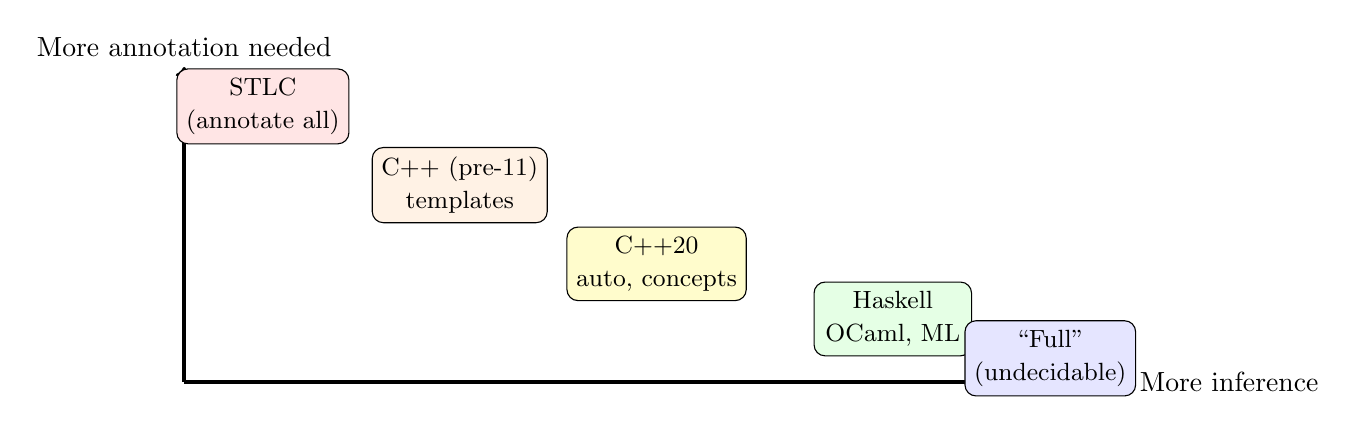
\begin{tikzpicture}[x=1cm, y=1cm]
  % Axis
  \draw[->, very thick] (0,0) -- (12,0) node[right] {More inference};
  \draw[->, very thick] (0,0) -- (0,4)  node[above] {More annotation needed};

  % Languages
  \node[draw, fill=red!10,   rounded corners, align=center, minimum width=2cm] at (1, 3.5)
    {\small STLC \\ \small (annotate all)};
  \node[draw, fill=orange!10,rounded corners, align=center, minimum width=2.2cm] at (3.5, 2.5)
    {\small C++ (pre-11)\\ \small templates};
  \node[draw, fill=yellow!20,rounded corners, align=center, minimum width=2cm] at (6, 1.5)
    {\small C++20 \\ \small \code{auto}, concepts};
  \node[draw, fill=green!10, rounded corners, align=center, minimum width=2cm] at (9, 0.8)
    {\small Haskell \\ \small OCaml, ML};
  \node[draw, fill=blue!10,  rounded corners, align=center, minimum width=2cm] at (11, 0.3)
    {\small ``Full'' \\ \small (undecidable)};
\end{tikzpicture}
\end{center}

\subsection{Advantages of More Inference}

\begin{itemize}
  \item \textbf{Less boilerplate.}
        You write the logic; the compiler fills in the types.
        Code is shorter and often easier to read.
  \item \textbf{Easier refactoring.}
        Change a type in one place; the inference engine propagates it
        everywhere (or points out inconsistencies).
  \item \textbf{Types as documentation that never lies.}
        Since the compiler checks them, inferred types are always correct.
\end{itemize}

\subsection{Disadvantages of More Inference}

\begin{itemize}
  \item \textbf{Harder error messages.}
        When inference fails, it can be far from where the actual mistake is.
        The error ``type mismatch between $\alpha$ and $\mathsf{int}$'' may
        appear in completely the wrong place.
  \item \textbf{Surprising types.}
        A small change to an expression can cause inference to pick a
        completely different type, possibly breaking other code.
  \item \textbf{Types as lost documentation.}
        If you omit annotations, reading the code does not tell you types.
        You must ask the IDE or the compiler.
  \item \textbf{Compilation speed.}
        Full unification over a large program is expensive.
        This is one reason C++ compilation is slow: template instantiation
        involves a lot of type computation.
\end{itemize}

\begin{warning}[The Monomorphism Restriction]
Haskell has a notorious pitfall called the \emph{monomorphism restriction}.
If you write a top-level binding without a type signature that ``looks like'' a
value (not a function), Haskell may infer a monomorphic type rather than the
polymorphic one you expect:

\begin{lstlisting}[style=haskell]
-- Without annotation, GHC may not generalise this:
defaultDouble = fromIntegral 42  -- could be Int, Integer, Double, ...
-- Error (or a type default): type variable is ambiguous

-- Fix: add a signature
defaultDouble :: Double
defaultDouble = fromIntegral 42  -- now unambiguous
\end{lstlisting}

The monomorphism restriction was designed to avoid accidentally recomputing
expensive values, but it surprises many newcomers.
It can be disabled with \code{\{-\# LANGUAGE NoMonomorphismRestriction \#-\}}.
\end{warning}

\subsection{The Sweet Spot}

Different languages make different trade-offs:

\begin{center}
\renewcommand{\arraystretch}{1.5}
\begin{tabular}{lll}
\toprule
\textbf{Language} & \textbf{Inference style} & \textbf{Annotation policy} \\
\midrule
Haskell / GHC & Full HM + extensions & Optional on top-level (recommended) \\
OCaml / F\# & HM & Optional, rarely needed \\
Rust & Local + HM-like & Required on function signatures \\
Swift & Local + bidirectional & Required on function signatures \\
C++ (modern) & Pattern-matching + \code{auto} & Required on function declarations \\
Go & Very limited (\code{:=}) & Mostly explicit \\
Java & Local (\code{var}) + generics & Mostly explicit \\
Python & None (optional hints) & Type hints are documentation only \\
\bottomrule
\end{tabular}
\end{center}

The consensus in language design today is roughly:
\begin{itemize}
  \item Infer inside function bodies.
  \item Require annotations on function signatures (they serve as interfaces).
  \item Handle generics/templates with some combination of inference and
        explicit arguments.
\end{itemize}

\begin{keyinsight}[Type Annotations Serve Multiple Masters]
A type annotation on a function signature is not just there to help the
compiler.
It serves as \emph{documentation} for human readers.
It provides a \emph{checkpoint}: if you know the type of a function is
$\mathsf{int} \to \mathsf{int}$ and you make changes that cause the compiler
to infer $\mathsf{double} \to \mathsf{double}$, the annotation catches the
mismatch immediately rather than propagating a subtle change silently through
the codebase.

Type annotations at module boundaries (function signatures, class members)
are nearly universally agreed to be good practice, even in languages that do
not require them.
\end{keyinsight}

% ------------------------------------------------------------
\section{A Deeper Dive: The Algorithm in Pseudocode}
\label{sec:algorithm-w-formal}
% ------------------------------------------------------------

For the more mathematically inclined reader, here is a more formal
pseudocode rendering of Algorithm~W.
We use the notation $\mathsf{ftv}(\tau)$ for the set of free type variables
in $\tau$, and $[\bar{\alpha} \mapsto \bar{\beta}]$ for substituting each
$\alpha_i$ with $\beta_i$.

\begin{lstlisting}[style=pseudocode]
-- Type scheme: forall [alpha_1, ..., alpha_n]. tau
data Scheme = Forall [TyVar] Type

-- A substitution: map from type variables to types
type Subst = Map TyVar Type

-- Apply a substitution to a type
apply : Subst -> Type -> Type
apply S (TyVar a)      = if a in S then S(a) else TyVar a
apply S (ty1 -> ty2)   = (apply S ty1) -> (apply S ty2)
apply S (List ty)      = List (apply S ty)
apply S BaseType       = BaseType   -- int, bool, etc.

-- Compose substitutions: (compose S2 S1)(x) = apply S2 (S1(x))
compose : Subst -> Subst -> Subst

-- Unification (Robinson's algorithm)
unify : Type -> Type -> Either TypeError Subst
unify (TyVar a)   t        | a not in ftv(t)  = {a |-> t}
unify t           (TyVar a)| a not in ftv(t)  = {a |-> t}
unify (TyVar a)   (TyVar a)                   = {}  -- delete
unify (s1 -> s2)  (t1 -> t2)                  =
    let S1 = unify s1 t1
        S2 = unify (apply S1 s2) (apply S1 t2)
    in  compose S2 S1
unify s t | s == t                            = {}  -- same base type
unify _ _                                     = error TypeError

-- Generalise: close over free type variables not in the environment
generalise : Env -> Type -> Scheme
generalise env tau =
    let free_in_tau = ftv(tau)
        free_in_env = union { ftv(scheme) | (x, scheme) in env }
        to_quantify = free_in_tau \ free_in_env  -- set difference
    in  Forall (list to_quantify) tau

-- Instantiate: replace universally-quantified vars with fresh ones
instantiate : Scheme -> Type
instantiate (Forall alphas tau) =
    let betas = { fresh() | alpha in alphas }
        subst = { alpha_i |-> beta_i | i in 1..n }
    in  apply subst tau

-- Algorithm W
W : Env -> Expr -> (Subst, Type)

W env (Var x) =
    let sigma = lookup x env  -- fails if not found
        tau   = instantiate sigma
    in  ({}, tau)

W env (Lit n) = ({}, Int)  -- for integer literals

W env (Lam x body) =
    let alpha     = fresh()
        env'      = extend env (x, Forall [] alpha)  -- monomorphic
        (S1, tau) = W env' body
    in  (S1, apply S1 alpha -> tau)

W env (App e1 e2) =
    let (S1, tau1) = W env e1
        (S2, tau2) = W (apply S1 env) e2
        beta       = fresh()
        S3         = unify (apply S2 tau1) (tau2 -> beta)
    in  (compose S3 (compose S2 S1), apply S3 beta)

W env (Let x e1 e2) =
    let (S1, tau1)  = W env e1
        env1        = apply S1 env
        sigma1      = generalise env1 tau1   -- <-- generalise here
        env2        = extend env1 (x, sigma1)
        (S2, tau2)  = W env2 e2
    in  (compose S2 S1, tau2)
\end{lstlisting}

This is the complete Algorithm~W.
In about 50 lines of pseudocode, you have a type inferencer for a
Hindley-Milner language.
Real implementations add error messages, source locations, pretty-printing,
and many language features, but the core is exactly this.

% ------------------------------------------------------------
\section{Summary of the Chapter}
\label{sec:ch6-summary}
% ------------------------------------------------------------

We have covered a lot of ground.
Here is a map of what we learned:

\begin{center}
\begin{tikzpicture}[
  node distance=1.5cm and 2.5cm,
  box/.style={draw, rounded corners, align=center, minimum width=3.2cm,
              minimum height=1.0cm, fill=blue!5},
  arrow/.style={->, thick, blue!60!black}
]
  \node[box] (prob) {Unannotated\\expression};
  \node[box, right=of prob] (cgen) {Constraint\\Generation};
  \node[box, right=of cgen] (uni)  {Unification\\(Robinson)};
  \node[box, right=of uni]  (type) {Principal\\Type};
  \node[box, below=of cgen] (letg) {Generalisation\\(\code{let})};
  \node[box, below=of uni]  (fail) {Type Error};

  \draw[arrow] (prob) -- (cgen);
  \draw[arrow] (cgen) -- (uni);
  \draw[arrow] (uni)  -- node[above]{\small success} (type);
  \draw[arrow] (uni)  -- node[right]{\small fail} (fail);
  \draw[arrow] (cgen) -- (letg);
  \draw[arrow] (letg) -- (uni);
\end{tikzpicture}
\end{center}

\begin{enumerate}
  \item \textbf{Annotation burden}: Writing types by hand in STLC and
        System~F is tedious. Inference automates this.
  \item \textbf{Constraint generation}: Walk the AST, assign fresh type
        variables, emit equations from language constructs.
  \item \textbf{Unification}: Robinson's algorithm solves systems of type
        equations. The occurs check prevents infinite types.
  \item \textbf{Algorithm W}: Combines constraint generation and unification.
        Returns the principal type or a type error.
  \item \textbf{Principal types}: The most general type that fits. HM always
        computes it.
  \item \textbf{Let-polymorphism}: The \code{let} construct introduces
        generalisation. Lambda-bound variables stay monomorphic.
  \item \textbf{C++ inference}: Template deduction and \code{auto} are limited
        forms of inference. Pattern matching, not full unification.
  \item \textbf{Limits}: Full System~F inference is undecidable (Wells, 1999).
        Higher-rank types require annotations.
  \item \textbf{Bidirectional checking}: Combines bottom-up synthesis and
        top-down checking. Handles higher-rank and dependent types.
  \item \textbf{Trade-offs}: More inference means less annotation but also
        harder errors and less explicit documentation.
\end{enumerate}

% ------------------------------------------------------------
\section{Exercises}
\label{sec:ch6-exercises}
% ------------------------------------------------------------

\begin{exercise}[Constraint Generation by Hand]
Manually generate constraints for the following expressions.
Show all fresh type variables and all equations produced.
\begin{enumerate}[label=(\alph*)]
  \item $\lambda x.\, \lambda y.\, x$
  \item $\lambda f.\, \lambda x.\, f\, x$
  \item $\lambda x.\, (x, x)$, where $(a, b)$ forms a pair of type
        $a \times b$.
  \item $\lambda x.\, \text{if } x \text{ then } 1 \text{ else } 0$
\end{enumerate}
\end{exercise}

\begin{exercise}[Unification by Hand]
Unify the following pairs of types, showing each step.
If unification fails, explain why.
\begin{enumerate}[label=(\alph*)]
  \item $\alpha \to \beta$ and $\mathsf{int} \to \mathsf{bool}$
  \item $\alpha \to \alpha$ and $\mathsf{int} \to \beta$
  \item $\mathsf{List}(\alpha)$ and $\mathsf{List}(\mathsf{int} \to \beta)$
  \item $\alpha \to \mathsf{int}$ and $\mathsf{bool} \to \alpha$
        (hint: what happens when you substitute?)
  \item $\alpha$ and $\mathsf{List}(\alpha)$ (occurs check)
\end{enumerate}
\end{exercise}

\begin{exercise}[Principal Types]
Determine the principal type of the following expressions.
Show your reasoning.
\begin{enumerate}[label=(\alph*)]
  \item $\lambda x.\, \lambda y.\, x\, y$
  \item $\lambda x.\, \lambda y.\, \lambda z.\, x\, z\, (y\, z)$
        (this is the $S$ combinator from combinatory logic)
  \item $\lambda x.\, (x, x\, 1)$ (can it be typed in HM?)
  \item \code{map} with definition
        $\mathit{map} = \lambda f.\, \lambda \ell.\,
        \text{if } \ell = [] \text{ then } []
        \text{ else } f\,(\mathit{head}\,\ell) :: \mathit{map}\, f\, (\mathit{tail}\,\ell)$
\end{enumerate}
\end{exercise}

\begin{exercise}[Let vs Lambda]
Explain in your own words why:
\begin{lstlisting}[style=haskell]
let id = \x -> x in (id 3, id True)
\end{lstlisting}
type-checks in Hindley-Milner, but:
\begin{lstlisting}[style=haskell]
(\id -> (id 3, id True)) (\x -> x)
\end{lstlisting}
does not (in standard HM without rank-2 extensions).

Then: what would need to change in the typing rules to make the second
version work?
(Hint: think about rank-2 types.)
\end{exercise}

\begin{exercise}[C++ Deduction]
For each of the following C++ calls, determine what the compiler deduces
for the template parameter(s), or explain why deduction fails:

\begin{lstlisting}[style=cpp]
template<typename T> T foo(T a, T b);
template<typename T, typename U> T bar(T a, U b);
template<typename T> void baz(std::vector<T> v);

// What are T, U in each call?
foo(1, 2);           // (a)
foo(1, 2.0);         // (b)
bar(1, 2.0);         // (c)
baz({1, 2, 3});      // (d) -- tricky!
foo(std::string{"hi"}, "world");  // (e)
\end{lstlisting}
\end{exercise}

\begin{exercise}[Implementing Mini-HM]
Implement a tiny Hindley-Milner type inferencer in the language of your
choice.
Your inferencer should handle:
\begin{itemize}
  \item Integer and boolean literals.
  \item Variables (looked up in an environment).
  \item Lambda abstractions $\lambda x.\, e$.
  \item Applications $e_1\; e_2$.
  \item Let bindings \textbf{let} $x = e_1$ \textbf{in} $e_2$.
\end{itemize}
Test it on: the identity function, the constant function
$\lambda x.\, \lambda y.\, x$, and double application
$\lambda f.\, \lambda x.\, f\,(f\,x)$.

Extra credit: implement the occurs check and produce a clear error message
when it triggers.
\end{exercise}

\begin{exercise}[Bidirectional Checking]
The following Rust function uses type inference:
\begin{lstlisting}[style=cpp]
fn apply<A, B>(f: impl Fn(A) -> B, x: A) -> B {
    f(x)
}
let result = apply(|x| x + 1, 42);
\end{lstlisting}
\begin{enumerate}[label=(\alph*)]
  \item What types are inferred for the closure \code{|x| x + 1}?
        In what order does Rust's type checker figure them out?
        (Top-down from the expected type of \code{f}, or bottom-up from the
        body?)
  \item Now consider: \code{let f: fn(i64) -> i64 = |x| x + 1;}
        How does this explicit type annotation change the inference?
        Which mode (checking or synthesis) is this an example of?
  \item What would happen if you wrote
        \code{let f = |x| x + 1;} without any context?
        What type does Rust give to \code{x}?
\end{enumerate}
\end{exercise}

% ------------------------------------------------------------
\begin{takeaway}[Chapter 6 Takeaways]
\begin{itemize}
  \item \textbf{Type inference automates annotation.}
        Instead of writing types by hand, a type inferencer works out what
        types must be from how expressions are used.

  \item \textbf{Constraint generation + unification = inference.}
        Walk the AST and emit type equations.
        Then solve those equations with Robinson's unification algorithm.

  \item \textbf{The occurs check prevents infinite types.}
        Before binding $\alpha$ to $\tau$, verify $\alpha$ does not appear
        inside $\tau$.
        Infinite types are unsound.

  \item \textbf{Algorithm W (Hindley-Milner) finds principal types.}
        It is sound, complete, and always computes the most general type.
        It is the gold standard for rank-1 polymorphism.

  \item \textbf{Let-polymorphism is the key to reusable inference.}
        \code{let}-bound variables are generalised to polymorphic schemes.
        Lambda-bound variables stay monomorphic within their scope.

  \item \textbf{C++ template deduction is limited pattern matching.}
        Not full unification. Fails in many cases that HM handles smoothly.
        \code{auto} and \code{decltype} extend it significantly.

  \item \textbf{Full System F inference is undecidable.}
        Wells (1999) proved it.
        Rank-2 types and higher require annotations.

  \item \textbf{Bidirectional checking handles what pure inference cannot.}
        Alternating between synthesis (bottom-up) and checking (top-down)
        handles higher-rank types, dependent types, and complex overloading.

  \item \textbf{Inference is a trade-off.}
        More inference means less boilerplate but harder errors and less
        explicit documentation.
        Most languages annotate function boundaries and infer locally.

  \item \textbf{Principal types make refactoring safe.}
        HM infers the most general type possible.
        Your code is automatically as reusable as it can be.
\end{itemize}
\end{takeaway}
